\documentclass[12pt]{article}

% Pacotes para o português.
\usepackage[utf8]{inputenc}
\usepackage[T1]{fontenc}

\usepackage{graphicx}     % Comando \includegraphics
\usepackage{xcolor}       % Comando de cores \textcolor
\usepackage{indentfirst}  % Indenta o primeiro parágrafo de cada seção
\usepackage{url}          % Comandos \url e \href
\usepackage[top=2cm, bottom=2cm, left=2cm, right=2cm]{geometry} % Define as margens do documento
\usepackage{multirow}     % Permite criar tabelas com uma célula ocupando várias linhas
\usepackage{amssymb}      % Símbolos matemáticos
\usepackage{amsmath}
\usepackage{gensymb}
\usepackage{caption}      % Para definir o estilo das legendas de figuras e tabelas.
\usepackage{setspace}     % Para definir espaçamento entre linhas. (\onehalfspacing, \singlespacing, \doublespacing)
\usepackage{breakcites}   % Para permitir quebra de linha no meio de citações.
\usepackage{times}        % Fonte Times New Roman
\usepackage{caption}
\usepackage{subcaption}
\usepackage{csvsimple}

% Comando para marcar o texto para revisão.
% \newcommand{\rev}[1]{\textcolor{red}{#1}}
\graphicspath{{./images/}}

\begin{document}
\doublespacing

\begin{titlepage}
    \begin{center}
        {\large \sc University of Toronto} \\
        {\large \sc Faculty of Applied Siences and Engineering}\\[0.7cm]
        {\small \sc Division of Engineering Science}
        
        \vspace{4cm}
        
        % Título.
        {\large \sc PHY180F}\\
        \rule{\linewidth}{2pt}
        
        \vspace{0.9em} % Ajuste ao seu gosto
        {\Large \bfseries Pendulum Lab - Final Report}
        \vspace{0.2em} % Ajuste ao seu gosto
        
        \rule{\linewidth}{2pt} \\
        {\small \sc December 9th, 2020}
    \end{center}
    
    \vspace{4cm}
    
    % Assinaturas
    \begin{minipage}{0.43\textwidth}
        \emph{Author:}
        Jayden Lefebvre\\
        UTorID:
        lefebv69
    \end{minipage}
    \hspace{1cm}
    \begin{minipage}{0.43\textwidth}
        \emph{Professor:}
        \hspace{1.5cm} Dr. Joseph Thywissen\\
        \emph{Teaching Assistant: }
        Mr. Saeed Oghbaey
    \end{minipage}
    
    \vfill
\end{titlepage}


\pagestyle{empty}
\tableofcontents
\newpage
\setcounter{page}{1}
\pagestyle{plain}
\singlespacing
\section{Introduction}
\label{section:intro}
The purpose of this lab is to investigate the factors that contribute to a pendulum's behaviour, with a specific focus on \emph{simple harmonic motion} (see Section \ref{section:motion}).
In order to determine the fitness of a pendulum to the simple harmonic motion model, I will be investigating the relationships between period of oscillation and initial amplitude (\ref{section:q3}), string length (\ref{section:q4a}), and bob mass (\ref{section:q4b}). 
In addition, I will be investigating the $Q$ factor or 'quality' of my pendulum (\ref{section:q2}).

\section{Background}
\label{section:background}
When released from some initial amplitude - angular displacement from equilibrium -  
the pendulum is acted upon by the component of gravity \emph{tangential} to the string. 
As it overshoots the equilibrium point and continues its oscillation, the tangential 
component of gravity continues to act as a \emph{restorative force}, attempting to bring the 
pendulum to rest at equilibrium. This continues until all energy in the system is dissipated, either via friction about the pin, or air resistance.

\subsection{Simple Harmonic Motion and Q Factor}
\label{section:motion}
Pendulums operate on the principle of \emph{simple harmonic motion}. 
In non-ideal pendulum, the amplitude of oscillation decreases over time. This energy dissipation is due to a \emph{damping force} (friction and air resistance).
A \emph{damped oscillator}, as it is called, that has a large \emph{quality factor} $Q$ retains its energy for a longer time, and as such oscillates for more periods. The amplitude of a damped oscillator over time is described by:\\
\begin{equation}
    \label{eqn:motion}
    \theta(t) = \theta_0e^{t/\tau}\cos(2\pi\frac tT + \phi_0)
\end{equation}
\noindent
where $t$ is the time elapsed, $\theta_0$ is the initial amplitude, $\tau$ is the damping factor, $T$ is the period, $\phi_0$ is the phase offset.
There are two ways in which to calculate $Q$ factor:
\begin{equation}
    Q_1=\pi \frac \tau T \text{ where $\tau$ and $T$ are the decay constant and period, respectively;}
    \label{eqn:Q1}
\end{equation}
\begin{equation}
    Q_2=2N\text{ where $N$ is the number of oscillations before }\theta(t)=\theta_Q=e^{-\pi/2}\theta_0 \approx 20\%\text{ of }\theta_0
    \label{eqn:Q2}
\end{equation}

\subsection{Amplitude vs Period}
\label{powerseries}
Theoretically, if a pendulum operates in accordance with simple harmonic motion (Section \ref{section:motion}) and is symmetrical, the oscillation \emph{should} have the following properties: 
\begin{enumerate}
    \item There should be \textbf{no} relationship between \emph{sign} of initial amplitude and period length (symmetry);
    \item There should be negligible relationship between \emph{magnitude} of initial amplitude and period.
\end{enumerate}
Thus, if period and initial amplitude are fit to the power series:
\begin{equation}
    \label{eqn:powerseries}
    T = A + B\theta_0 + C \theta_0^2 + \cdots
\end{equation}
\noindent
B should be equal to experimental zero, and C should be reasonably zero for small initial amplitudes. \textbf{Note:} degrees higher than 2 are not used for the purposes of this lab.
\pagebreak
\subsection{Length vs Period}
\label{powerlaw}
If a pendulum operates in accordance with simple harmonic motion (Section \ref{section:motion}), the period of oscillation \emph{should} be proportional to the square root of the length (the distance from the axis of rotation to the center of mass, or COM):
$$
T \approx 2\sqrt{L}
$$
Expressed as an exponential function:
\begin{equation}
    \label{eqn:powerlaw}
    T = k(L_0 + L)^n
\end{equation}
\noindent
where $T$ is the period, $k$ is the coefficient (related to the restorative force, gravity), $n$ is the exponent, and $L_0$ is the "error" of our estimation for length (should be experimentally zero).

\section{Method}
\label{section:method}
\subsection{Apparatus Details}
\label{section:materials}
Despite the report requirement for \textbf{no materials list}, there is a general understanding of certain components of the pendulum apparatus that are vital to understanding the method:
\begin{itemize}
    \item The bob used is a container of small removable masses with a sturdy lid to which the string can be affixed;
    \item The string used is not stretchy, and is made of wound plastic fibers;
\end{itemize}
\subsection{Setup}
\label{section:setup}
\noindent
The apparatus setup is as follows:

\begin{enumerate}
    \item A mounting screw is installed at a fixed, sturdy mounting location;
    \item The bob is configured for the test (see below) and attached to string via self-tightening slipknot (see Appendix Figure \ref{appendix:setup} for a closer look);
    \item Non-slipping bowline knots are made in the string at fixed distances from the bob COM: 44.75", 39", 34.25", 29", and 25.25";
    \item Horizontal reference is placed \emph{in plane} with the pendulum oscillation (see Appendix Figure \ref{appendix:table});
    \item Tape marks are made at center (aka. pendulum equilibrium) on the horizontal reference, as well as 2ft (0.610m) in either direction (see Appendix Figure \ref{appendix:table});
    \item Camera is set up on camera stand, in plane with pendulum oscillation, with the bottom of the camera viewport calibrated to the horizontal reference (see Appendix Figure \ref{appendix:table});
\end{enumerate}
\pagebreak
\noindent
The pendulum is configured on a \emph{per-test basis}.\\

If the test requires the \emph{mass} be adjusted:
\begin{enumerate}
    \item Remove the cap from the bob;
    \item Pour some of the pendulum's mass into a sturdy container;
    \item Place the bob on the scale, and record the bob mass, adjust mass again if necessary;
    \item Replace the cap and ensure the bob is tied to the string (as described above);
\end{enumerate}
\noindent
If the test requires the \emph{length} be adjusted, loop the selected bowline around the fixed mounting screw.

\subsection{Video Capture}
\label{section:videocapture}
\noindent
3 sets of videos were taken:
\begin{enumerate}
    \item \textbf{Full Period} - Pendulum (mass 2032g, length 34.25") released at 90$\deg$, allowed to decay to <15$\deg$;
    \item \textbf{String Length Trials} - Pendulum (mass 2032g) released at a moderate angle (think 30$\deg$-50$\deg$) with varying string length (44.75", 39", 34.25", 29", 25.25"), allowed to oscillate for 4-6 periods;
    \item \textbf{Bob Mass Trials} - Pendulum (length 34.25") released at a moderate angle (think 30$\deg$-50$\deg$) with varying bob mass (2032g, 1784g, 1607g, 1366g, 1012g), allowed to oscillate for 4-6 periods;
\end{enumerate}
\subsection{Tracker Video Analysis}
\label{section:trackeranalysis}
The Tracker Video Analysis and Modelling Tool\cite{tracker} was used to track the position of the pendulum in the video captures across time.\\

\noindent
Preparing the video capture for Tracker software:
\begin{enumerate}
    \item In VLC, select "File > Convert / Stream" and open the video capture;
    \item Select "Custom" profile, customize with no audio track (minimize file size) and FLV encapsulation (Tracker compatibility);
    \item Save as a file with appropriate name;
\end{enumerate}
\noindent
Opening the video in Tracker software:
\begin{enumerate}
    \item In Tracker, select "File > Open File" and open the FLV video capture;
    \item Wait for all frames to be loaded;
\end{enumerate}
\pagebreak
\noindent
Calibrating the Tracker environment:
\begin{enumerate}
    \item Select "Track > New > Calibration Tools > Calibration Stick" and follow the Tracker's instructions to calibrate the ends of the stick to the center and 2ft marking on the horizontal reference in the video;
    \item Toggle "Track > Axes > Visible" \textbf{ON}, and drag the origin of the axes to the pendulum axis;
\end{enumerate}
\noindent
Tracking the pendulum:
\begin{enumerate}
    \item Select "Track > New > Point Mass";
    \item On the "Track Control" panel, select the new point mass (should be named "mass A") and select "Autotracker";
    \item Ensure the frame advance number in the bottom right of the screen is set to 5 (reduce total frames);
    \item Depending on the speed of the pendulum, you will have to switch between \emph{manually} tracking the pendulum frame-by-frame (Shift+LClick) or using the \emph{autotracker} (set keyframe position, template region, search region, and evolution rate, I used 60\%) and allowing it to search for you;
    \item Track the pendulum across all frames.
\end{enumerate}
\noindent
Exporting data for analysis:
\begin{enumerate}
    \item In the table panel (right side, bottom panel), click the table button and ensure x, y, theta r, and v are toggled on
    \item Right click inside the table, select "Numbers > Units..." and ensure that "Angle Units" is set to radians
    \item Left click inside the table, press "CMD+A" on Mac (or "CTRL+A" on Windows) to select the entire table
    \item Press "CMD+C" on Mac (or "CTRL+C" on Windows) to copy the entire table
    \item Paste the data into Google Sheets. You can now perform analysis on the data.
\end{enumerate}
\subsection{Python Data Analysis}
Scripts were written in the \emph{Python} programming language\cite{python} to calculate and plot the fits and residuals for each test. The \emph{SciPy}\cite{scipy} and \emph{matplotlib}\cite{matplotlib} libraries were used. Scripts can be found in Appendix Section \ref{appendix:scripts}.
\pagebreak
\subsection{Uncertainty}
\label{section:uncertainty}

\subsubsection{Measurement Uncertainties}
\noindent
There were numerous sources of measurement uncertainty, examined here:
\begin{itemize}
    \item Time - 60fps, assume $\pm$1 frame, $\pm$0.01667s
    \item Position (Reference Frame) - 2ft markers on table used as reference (Fig), my standard imperial measuring tape has $\pm$1/16in uncertainty, or 0.2\% positional uncertainty. This distance is used as the reference length when analyzing the footage in Tracker. Since all positions are measured as distances, all positional data would have this uncertainty.
    \item Position (Motion Blur) - Speed at apex when 2030g pendulum released from $\pi/2$rad is 4.042 m/s, which produced a motion blur in the video (Fig). The circular cross-section of the bob has a circumference of 10 5/8" = 26.988cm, or an actual diameter of 8.59cm which, due to motion blur, appeared to be 10.4cm on camera, corresponding to (10.4-8.59)/2 = 0.905cm of positional uncertainty. $v/v_0 * 0.905 / 100$
    \item Mass Uncertainty - $\pm$1g kitchen scale
\end{itemize}

The maximum of the two positional uncertainties are used per datum, per the uncertianty propagation conventions outlined in the Pendulum Lab Handout.

\subsubsection{Calculated Uncertainties}

Measurement uncertainty was propagated per the uncertianty propagation conventions outlined in the Pendulum Lab Handout.\\

In order to calculate uncertainty for angle measurements generated from positional data, the difference between the maximum and minimum angles for position $(x,y)$ - given uncertainties $x'$ and $y'$ is used. For example, consider the set of all 4 possible combinations:

$$ S = \{\arctan(\frac{y\pm y'}{x \pm x'} \cdots)\}$$

The numerical difference between the maximum and minimum possible angles for a given position is used as the angular uncertainty:

$$ \theta' = \max\{S\} - \min\{S\}$$

\subsubsection{General Limitations}
\noindent
There were several sources of uncalulable or irreducable uncertainties, here viewed as limitations:

\begin{itemize}
    \item Video pixellation leads to innacuracy in tracking;
    \item Autotracker has limited accuracy when estimating bob mass position;
    \item Video framerate (as well as Tracker frame step multiplier) limit time accuracy;
\end{itemize}

\newpage

\section{Results and Analysis}

\subsection{Q Factor}
\label{section:q2}
\subsubsection{Graphs}

\begin{figure}[h]
    \centering
    \begin{subfigure}[b]{0.48\textwidth}
        \centering
        \includegraphics[width=\textwidth]{q2_fit.png}
        \caption{Fit of data to decaying sinusoid (see Section \ref{section:q2fit}).}
        \label{fig:q2fit}
    \end{subfigure}
    \hfill
    \begin{subfigure}[b]{0.48\textwidth}
        \centering
        \includegraphics[width=\textwidth]{q2_residuals.png}
        \caption{Residuals of fit.}
        \label{fig:q2residuals}
    \end{subfigure}
    \hfill
    \caption{Pendulum swing data (2030g, 34.25"). \\Note that error bars are \emph{very} small.}
    \label{fig:q2fig}
\end{figure}
\subsubsection{Decaying Sinusoid Fit}
\label{section:q2fit}

The pendulum's amplitude over time bounded by $t \approx [80,130]$sec is shown in Figure \ref{fig:q2fit}, along with the fit of a decaying sinusoid as described in Equation \ref{eqn:motion}.
The specific values found by the curve fit function are as follows:
\begin{center}
    $
    \theta_0= 1.28 \pm 0.04\text{rad}$\\$
    \tau= 240 \pm 20\text{sec}^{-1}$\\$
    T= 2.1577 \pm 0.0002\text{sec}$\\$
    \phi_0= 21.98 \pm 0.03\text{rad}
    $
\end{center}
The specific equation for this fit is thus:
\begin{equation}
    \theta(t) = 1.28e^{t/240}\cos(2\pi\frac t{2.1577} + 21.98)
\end{equation}

\subsubsection{Calculating Q Factor}

\begin{equation}
    \label{eqn:Q1calc}
    Q1 = \pi \frac \tau T =\pi*\frac{242.01}{2.1577} = 350 \pm 30
\end{equation}
\begin{equation}
    \label{eqn:Q2calc}
    \theta_Q = \theta_0*e^{-\pi/2} = 0.295\pm0.009\text{rad}
\end{equation}
The above amplitude occurs after 126 full oscillations, meaning that according to Equation \ref{eqn:Q2}, $Q2 = 352$.\medskip\\

Given that $Q2$ is well within the uncertainty of $Q1$, I am \emph{very} confident about the accuracy of this number.

\pagebreak

\subsection{Amplitude vs Period}
\label{section:q3}
\subsubsection{Graphs}
\begin{figure}[h]
    \centering
    \begin{subfigure}[b]{0.48\textwidth}
        \centering
        \includegraphics[width=\textwidth]{q3_fit.png}
        \caption{Fit of amplitude vs period to power series (see Section \ref{section:q3fit}).}
        \label{fig:q3fit}
    \end{subfigure}
    \hfill
    \begin{subfigure}[b]{0.48\textwidth}
        \centering
        \includegraphics[width=\textwidth]{q3_residuals.png}
        \caption{Residuals of fit.}
        \label{fig:q3residuals}
    \end{subfigure}
    \hfill
    \caption{Pendulum swing data (2030g, 34.25"). \\Note that error bars are visible, but again \emph{very} small.}
    \label{fig:q3fig}
\end{figure}
\subsubsection{Power Series Fit}
\label{section:q3fit}

The pendulum's period over varying initial amplitude bounded by $\theta_0 \approx [-\pi/2,\pi/2]$rad is shown in Figure \ref{fig:q3fit}, along with the fit of a power series as described in Equation \ref{eqn:powerseries}.
The specific values found by the curve fitting function are as follows:
\begin{center}
    $
    A= 2.05 \pm 0.01\text{sec}
    $\\
    $
    B= 0.006 \pm 0.01 \frac {\text{sec}}{\text{rad}}\approx 0$\\
    $
    C= 0.11 \pm 0.02\frac {\text{sec}}{\text{rad}^2}
    $
\end{center}
The specific equation for this fit is thus:
\begin{equation}
    T = 2.05 + 0.11\theta_0^2
\end{equation}

\subsubsection{Symmetry Test}

Given that the value of $B$ is less than its uncertainty, it can be said to be "experimentally zero". 
As such, my pendulum passes the "asymmetry test", and is sufficiently symmetrical for further experimentation.\medskip\\

\pagebreak

\subsection{Length vs Period}
\label{section:q4a}
\subsubsection{Graphs}
\begin{figure}[h]
    \centering
    \begin{subfigure}[b]{0.48\textwidth}
        \centering
        \includegraphics[width=\textwidth]{q4a_fit.png}
        \caption{Fit of length vs period to power series (see Section \ref{section:q4afit}).}
        \label{fig:q4afit}
    \end{subfigure}
    \hfill
    \begin{subfigure}[b]{0.48\textwidth}
        \centering
        \includegraphics[width=\textwidth]{q4a_residuals.png}
        \caption{Residuals of fit.}
        \label{fig:q4aresiduals}
    \end{subfigure}
    \label{fig:q4afig}
\end{figure}
\begin{figure}[h]
    \centering
    \begin{subfigure}[b]{0.48\textwidth}
        \centering
        \includegraphics[width=\textwidth]{q4a_logfit.png}
        \caption{Fit of data to power law (see Section \ref{section:q4afit}, logarithmic axes).}
        \label{fig:q4alogfit}
    \end{subfigure}
    \hfill
    \begin{subfigure}[b]{0.48\textwidth}
        \centering
        \includegraphics[width=\textwidth]{q4a_logresiduals.png}
        \caption{Residuals of fit (logarithmic axes).}
        \label{fig:q4alogresiduals}
    \end{subfigure}
    \hfill
    \caption{Pendulum swing data (2030g) for varying lengths (44.75", 39", 34.25", 29", 25.25"). Note that residuals are far smaller than uncertainties.}
    \label{fig:q4alogfig}
\end{figure}
\subsubsection{Power Law Fit}
\label{section:q4afit}

The pendulum's period over varying length bounded by $L = [44.75, 39, 34.25, 29, 25.25]$ inches, or\\
$L=[1.137, 0.991, 0.870, 0.737, 0.641]$ meters is shown in Figure \ref{fig:q4afit}, along with the fit of a power law function as described in Equation \ref{eqn:powerlaw}.
The specific values found by the curve fitting function are as follows:
\begin{center}
    $
    k= 1.12 \pm 0.09
    $\\
    $
    L_0= -0.2 \pm 0.2 \text{m}\approx 0$\\
    $
    n= 0.4 \pm 0.1
    $
\end{center}
The specific equation for this fit is thus:
\begin{equation}
    T = 1.12L^{0.4}
\end{equation}

\subsubsection{Accuracy}

The exponent $n$ seems to be farther from $1/2$ than anticipated. When k is removed from the curve fitting parameters and fixed to 1:\\
$L_0: 0.06940995886640021$
$n: 0.5304151670699991$

$n$ is much closer to $1/2$, and $L_0$ is actually \emph{smaller} in magnitude. Since the addition of a coefficient makes the results less accurate to theory, perhaps more data points would have made the fit better.

\subsection{Period vs Mass}
\label{section:q4b}
\subsubsection{Graphs - Motion for Varying Mass}
\begin{figure}[h]
    \centering
    \begin{subfigure}[b]{0.48\textwidth}
        \centering
        \includegraphics[width=6cm,height=6cm, keepaspectratio]{q4b_fit1.png}
        \caption{Fit of pendulum motion with mass \textbf{2032g} to decaying sinusoid (see Section \ref{section:q2fit}).}

    \end{subfigure}
    \hfill
    \begin{subfigure}[b]{0.48\textwidth}
        \centering
        \includegraphics[width=6cm,height=6cm, keepaspectratio]{q4b_residuals1.png}
        \caption{Residuals of fit.}

    \end{subfigure}
    \begin{subfigure}[b]{0.48\textwidth}
        \centering
        \includegraphics[width=6cm,height=6cm, keepaspectratio]{q4b_fit2.png}
        \caption{Fit of pendulum motion with mass \textbf{1784g} to decaying sinusoid (see Section \ref{section:q2fit}).}

    \end{subfigure}
    \hfill
    \begin{subfigure}[b]{0.48\textwidth}
        \centering
        \includegraphics[width=6cm,height=6cm, keepaspectratio]{q4b_residuals2.png}
        \caption{Residuals of fit.}

    \end{subfigure}
    \label{fig:q4bfig1}
    \caption{Pendulum motion for varying mass, group 1.}
\end{figure}
\pagebreak
\begin{figure}[h]
    \centering
    \begin{subfigure}[b]{0.48\textwidth}
        \centering
        \includegraphics[width=\textwidth]{q4b_fit3.png}
        \caption{Fit of pendulum motion with mass \textbf{1607g} to decaying sinusoid (see Section \ref{section:q2fit}).}
    \end{subfigure}
    \hfill
    \begin{subfigure}[b]{0.48\textwidth}
        \centering
        \includegraphics[width=\textwidth]{q4b_residuals3.png}
        \caption{Residuals of fit.}
    \end{subfigure}
    \begin{subfigure}[b]{0.48\textwidth}
        \centering
        \includegraphics[width=6cm,height=6cm, keepaspectratio]{q4b_fit4.png}
        \caption{Fit of pendulum motion with mass \textbf{1366g} to decaying sinusoid (see Section \ref{section:q2fit}).}
    \end{subfigure}
    \hfill
    \begin{subfigure}[b]{0.48\textwidth}
        \centering
        \includegraphics[width=6cm,height=6cm, keepaspectratio]{q4b_residuals4.png}
        \caption{Residuals of fit.}
    \end{subfigure}
    \begin{subfigure}[b]{0.48\textwidth}
        \centering
        \includegraphics[width=6cm,height=6cm, keepaspectratio]{q4b_fit5.png}
        \caption{Fit of pendulum motion with mass \textbf{1012g} to decaying sinusoid (see Section \ref{section:q2fit}).}
    \end{subfigure}
    \hfill
    \begin{subfigure}[b]{0.48\textwidth}
        \centering
        \includegraphics[width=6cm,height=6cm, keepaspectratio]{q4b_residuals5.png}
        \caption{Residuals of fit.}
    \end{subfigure}
    \hfill
    \caption{Pendulum motion for varying mass, group 2.}
    \label{fig:q4bfig2}
\end{figure}
\pagebreak
\subsubsection{Period for Varying Mass}
\label{section:q4bsummary}
When the period is found for the pendulum with varying mass, values for $~\tau$ and $T$ are found, and are displayed in the following table:
\begin{center}
    \begin{tabular}{||c c c c c c||} 
        \hline
        Trial \# & Mass (g) & T (sec) & T' ($\pm$sec) & $\tau$ (sec$^{-1}$) & $\tau'$ ($\pm$sec$^{-1}$) \\ [0.5ex] 
        \hline\hline
        1 & 2032 & 1.939 & 0.001 & 150 & 40 \\ 
        \hline
        2 & 1784 & 1.945 & 0.001 & 200 & 100 \\
        \hline
        3 & 1607 & 1.9360 & 0.0006 & 200 & 40 \\
        \hline
        4 & 1366 & 1.9641 & 0.0009 & 300 & 100 \\
        \hline
        5 & 1012 & 1.9625 & 0.0009 & 130 & 30 \\ [1ex] 
        \hline
    \end{tabular}
\end{center}
\noindent
Values for $\theta_0$ and $\phi_0$ are ignored, as they relate more to where in the oscillation the recording starts, rather than the properties of the oscillator.\\
\noindent
A fit for period vs mass can be found below.
\begin{figure}[h]
    \centering
    \begin{subfigure}[b]{0.48\textwidth}
        \centering
        \includegraphics[width=\textwidth]{q4b_summaryfit.png}
        \caption{Fit of period vs varying mass to power series (See Equation \ref{eqn:powerseries}).}
        \label{fig:q4bfitsummary}
    \end{subfigure}
    \hfill
    \begin{subfigure}[b]{0.48\textwidth}
        \centering
        \includegraphics[width=\textwidth]{q4b_summaryresiduals.png}
        \caption{Residuals of fit.}
        \label{fig:q4bresidualssummary}
    \end{subfigure}
    \label{fig:q4bfigsummary}
\end{figure}
\pagebreak

\subsubsection{Analysis}
\noindent
The power series fit (Equation \ref{eqn:powerseries}) for mass vs period in Section \ref{section:q4bsummary} produced the following values:
\begin{center}
$A= 2.01 \pm 0.10$\\
$B= -0.00005 \pm 0.0001 \approx 0$\\
$C= 6\times 10^{-9} \pm 4\times 10^{-8}\approx 0$
\end{center}
Both $B$ and $C$ are experimentally zero. In addition, the magnitudes of $C$ and $B$ are \emph{tiny} in comparison to the values being examined ($1.935\leq T \leq 1.985$), and the uncertainties for the data points lie far from the line of best fit.\\
\noindent
For these reasons, seems to be \emph{no correlation} (linear or quadratic) between bob mass and period of oscillation.

\section{Conclusion}
\label{section:conclusion}

In Section \ref{section:q2}, I found that the Q factor of this pendulum is $Q=350$. This speaks to a high quality pendulum, meaning that it does not dissipate energy very quickly, and is able to oscillate for a long period of time. 
In Section \ref{section:q3}, I found that my pendulum is symmetrical. I also found that at amplitudes exceeding $\pm1.0$rad, the period begins to increase drastically. 
In Section \ref{section:q4a}, I found that my pendulum obeys similar laws to those expected, with a periodicity proportional to the root of the string length.
In Section \ref{section:q4b}, I found that the period of my pendulum is not correlated to the bob mass.\\

Overall, the pendulum I have constructed seems to closely match the "ideal" pendulum.

\pagebreak
\appendix
\section{Supplementary Photos}
\label{section:setup}

\begin{figure}[h]
    \centering
    \begin{subfigure}[b]{0.48\textwidth}
        \centering
        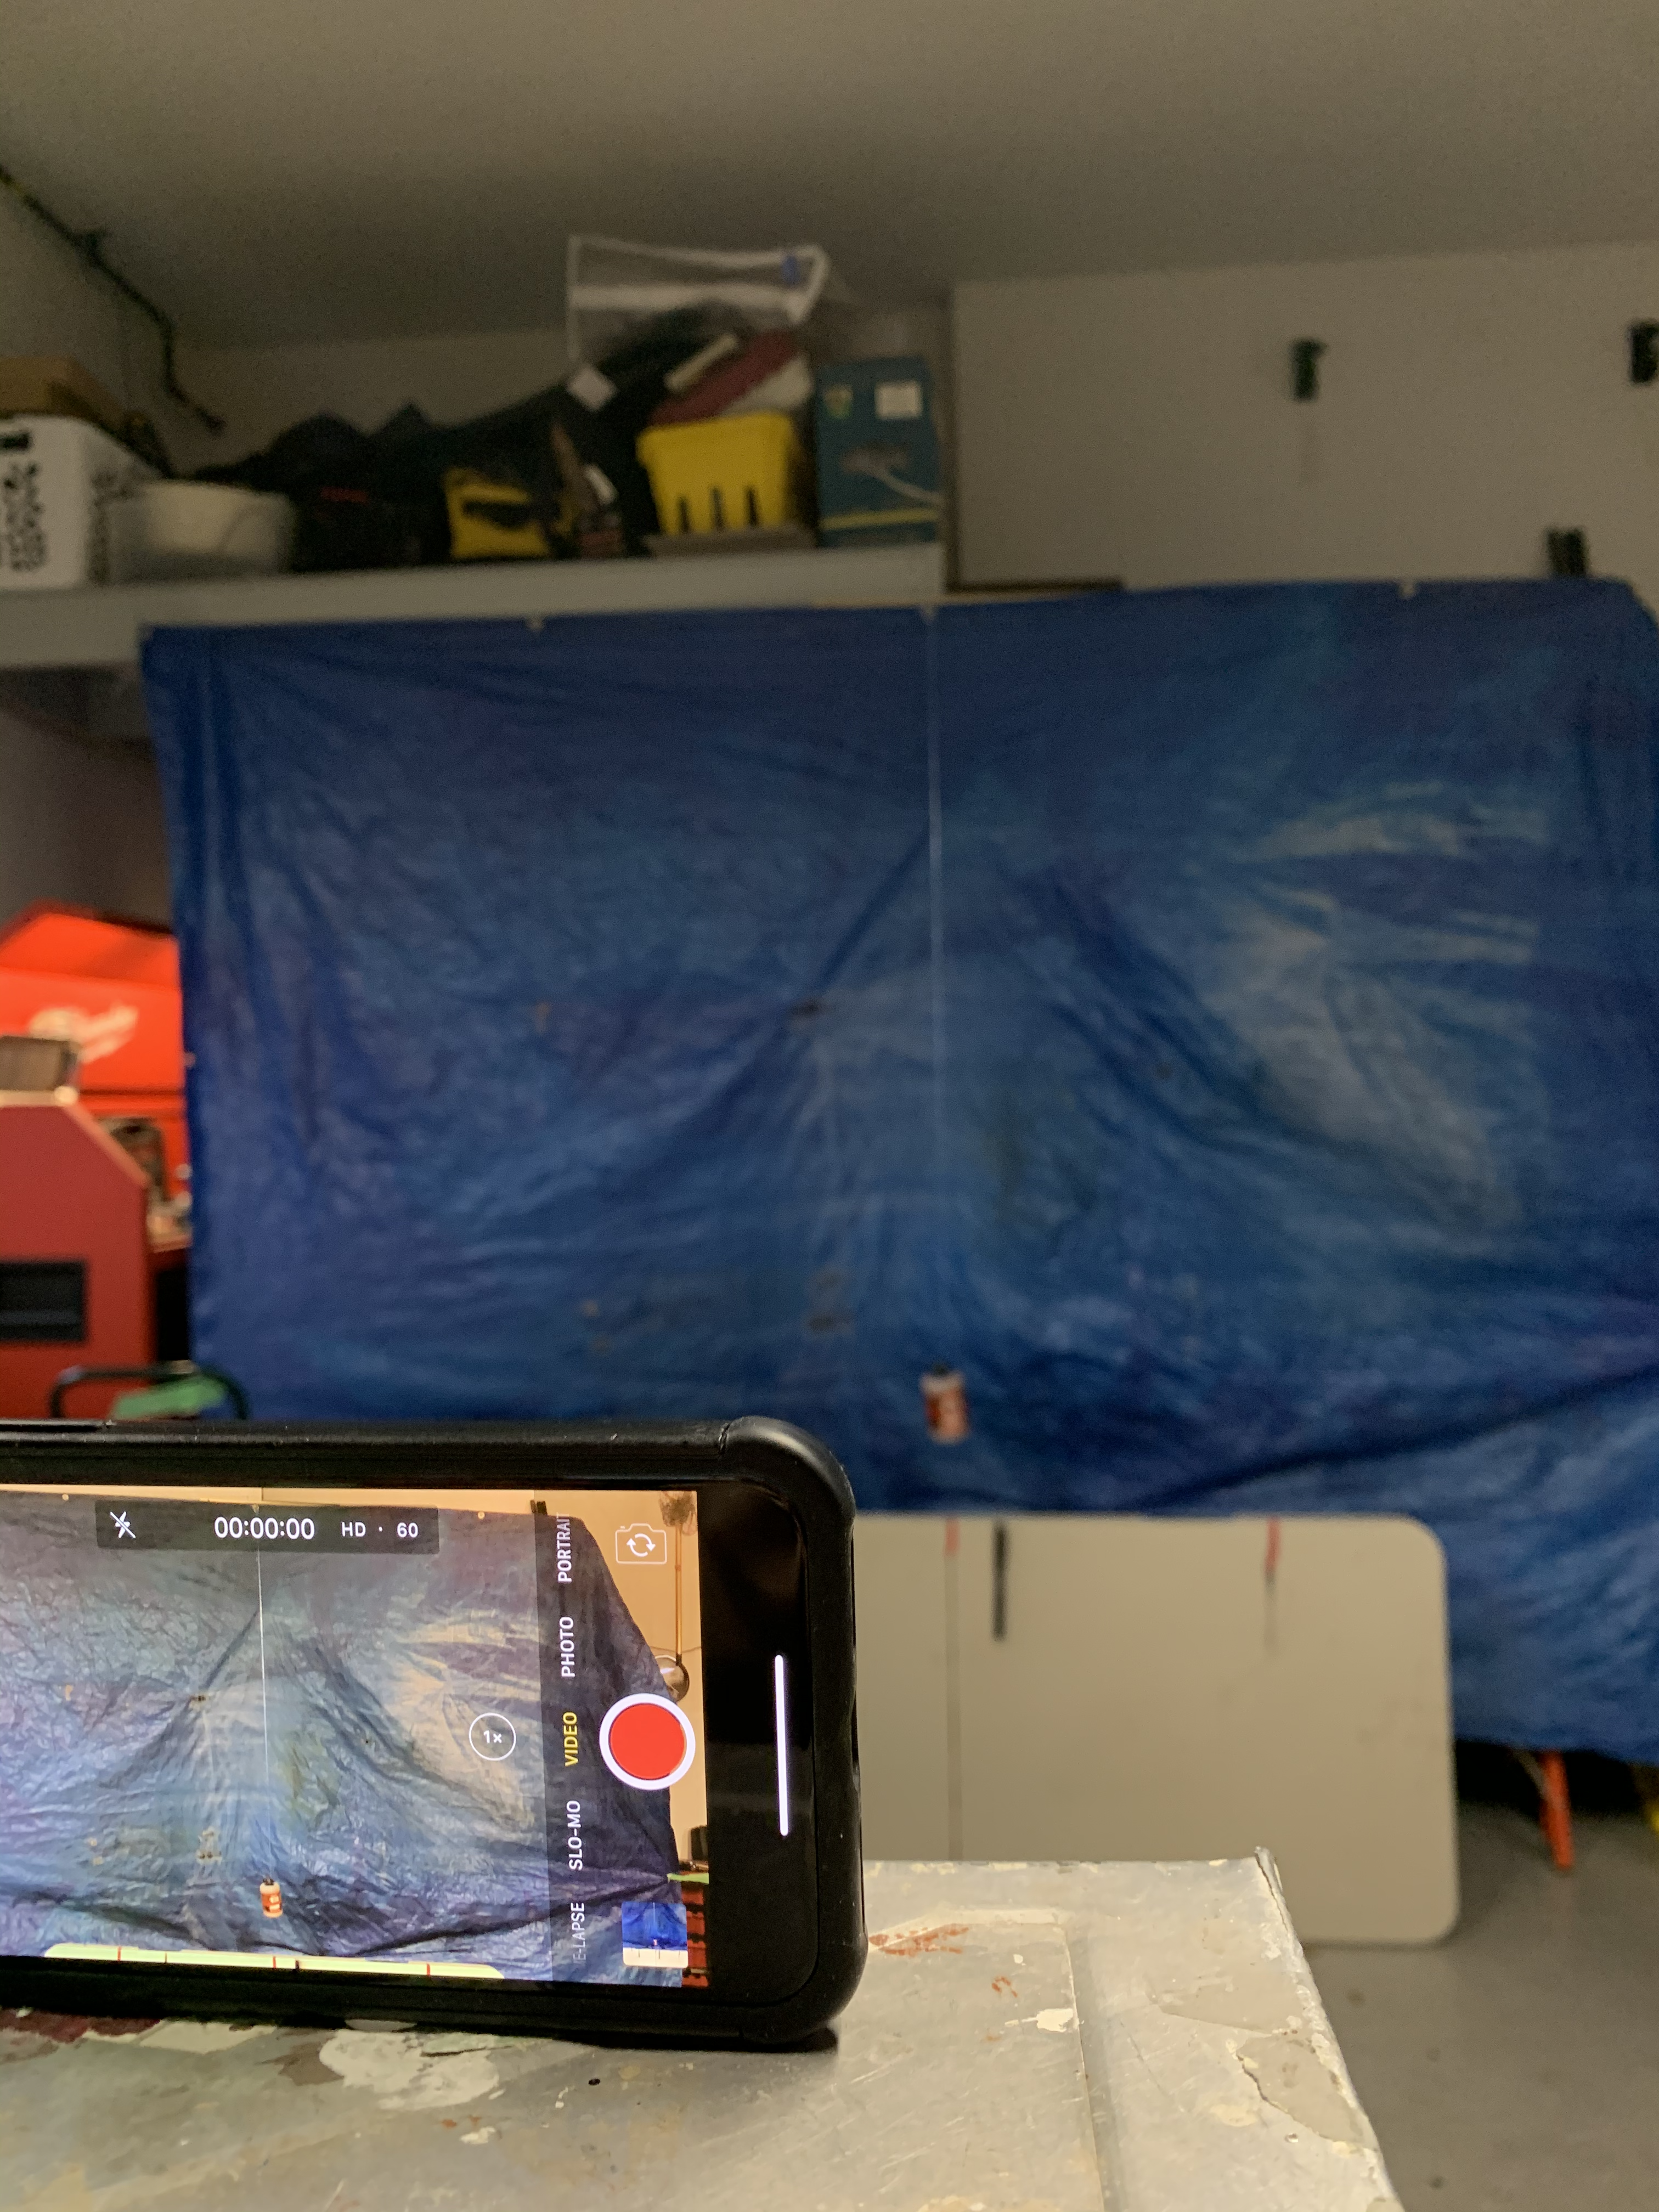
\includegraphics[width=6cm,height=6cm,keepaspectratio]{camera.png}
        \caption{View from the camera's perspective, showing the table as horizontal reference in the bottom of the camera viewport.}
        \label{appendix:camera}
    \end{subfigure}
    \hfill
    \begin{subfigure}[b]{0.48\textwidth}
        \centering
        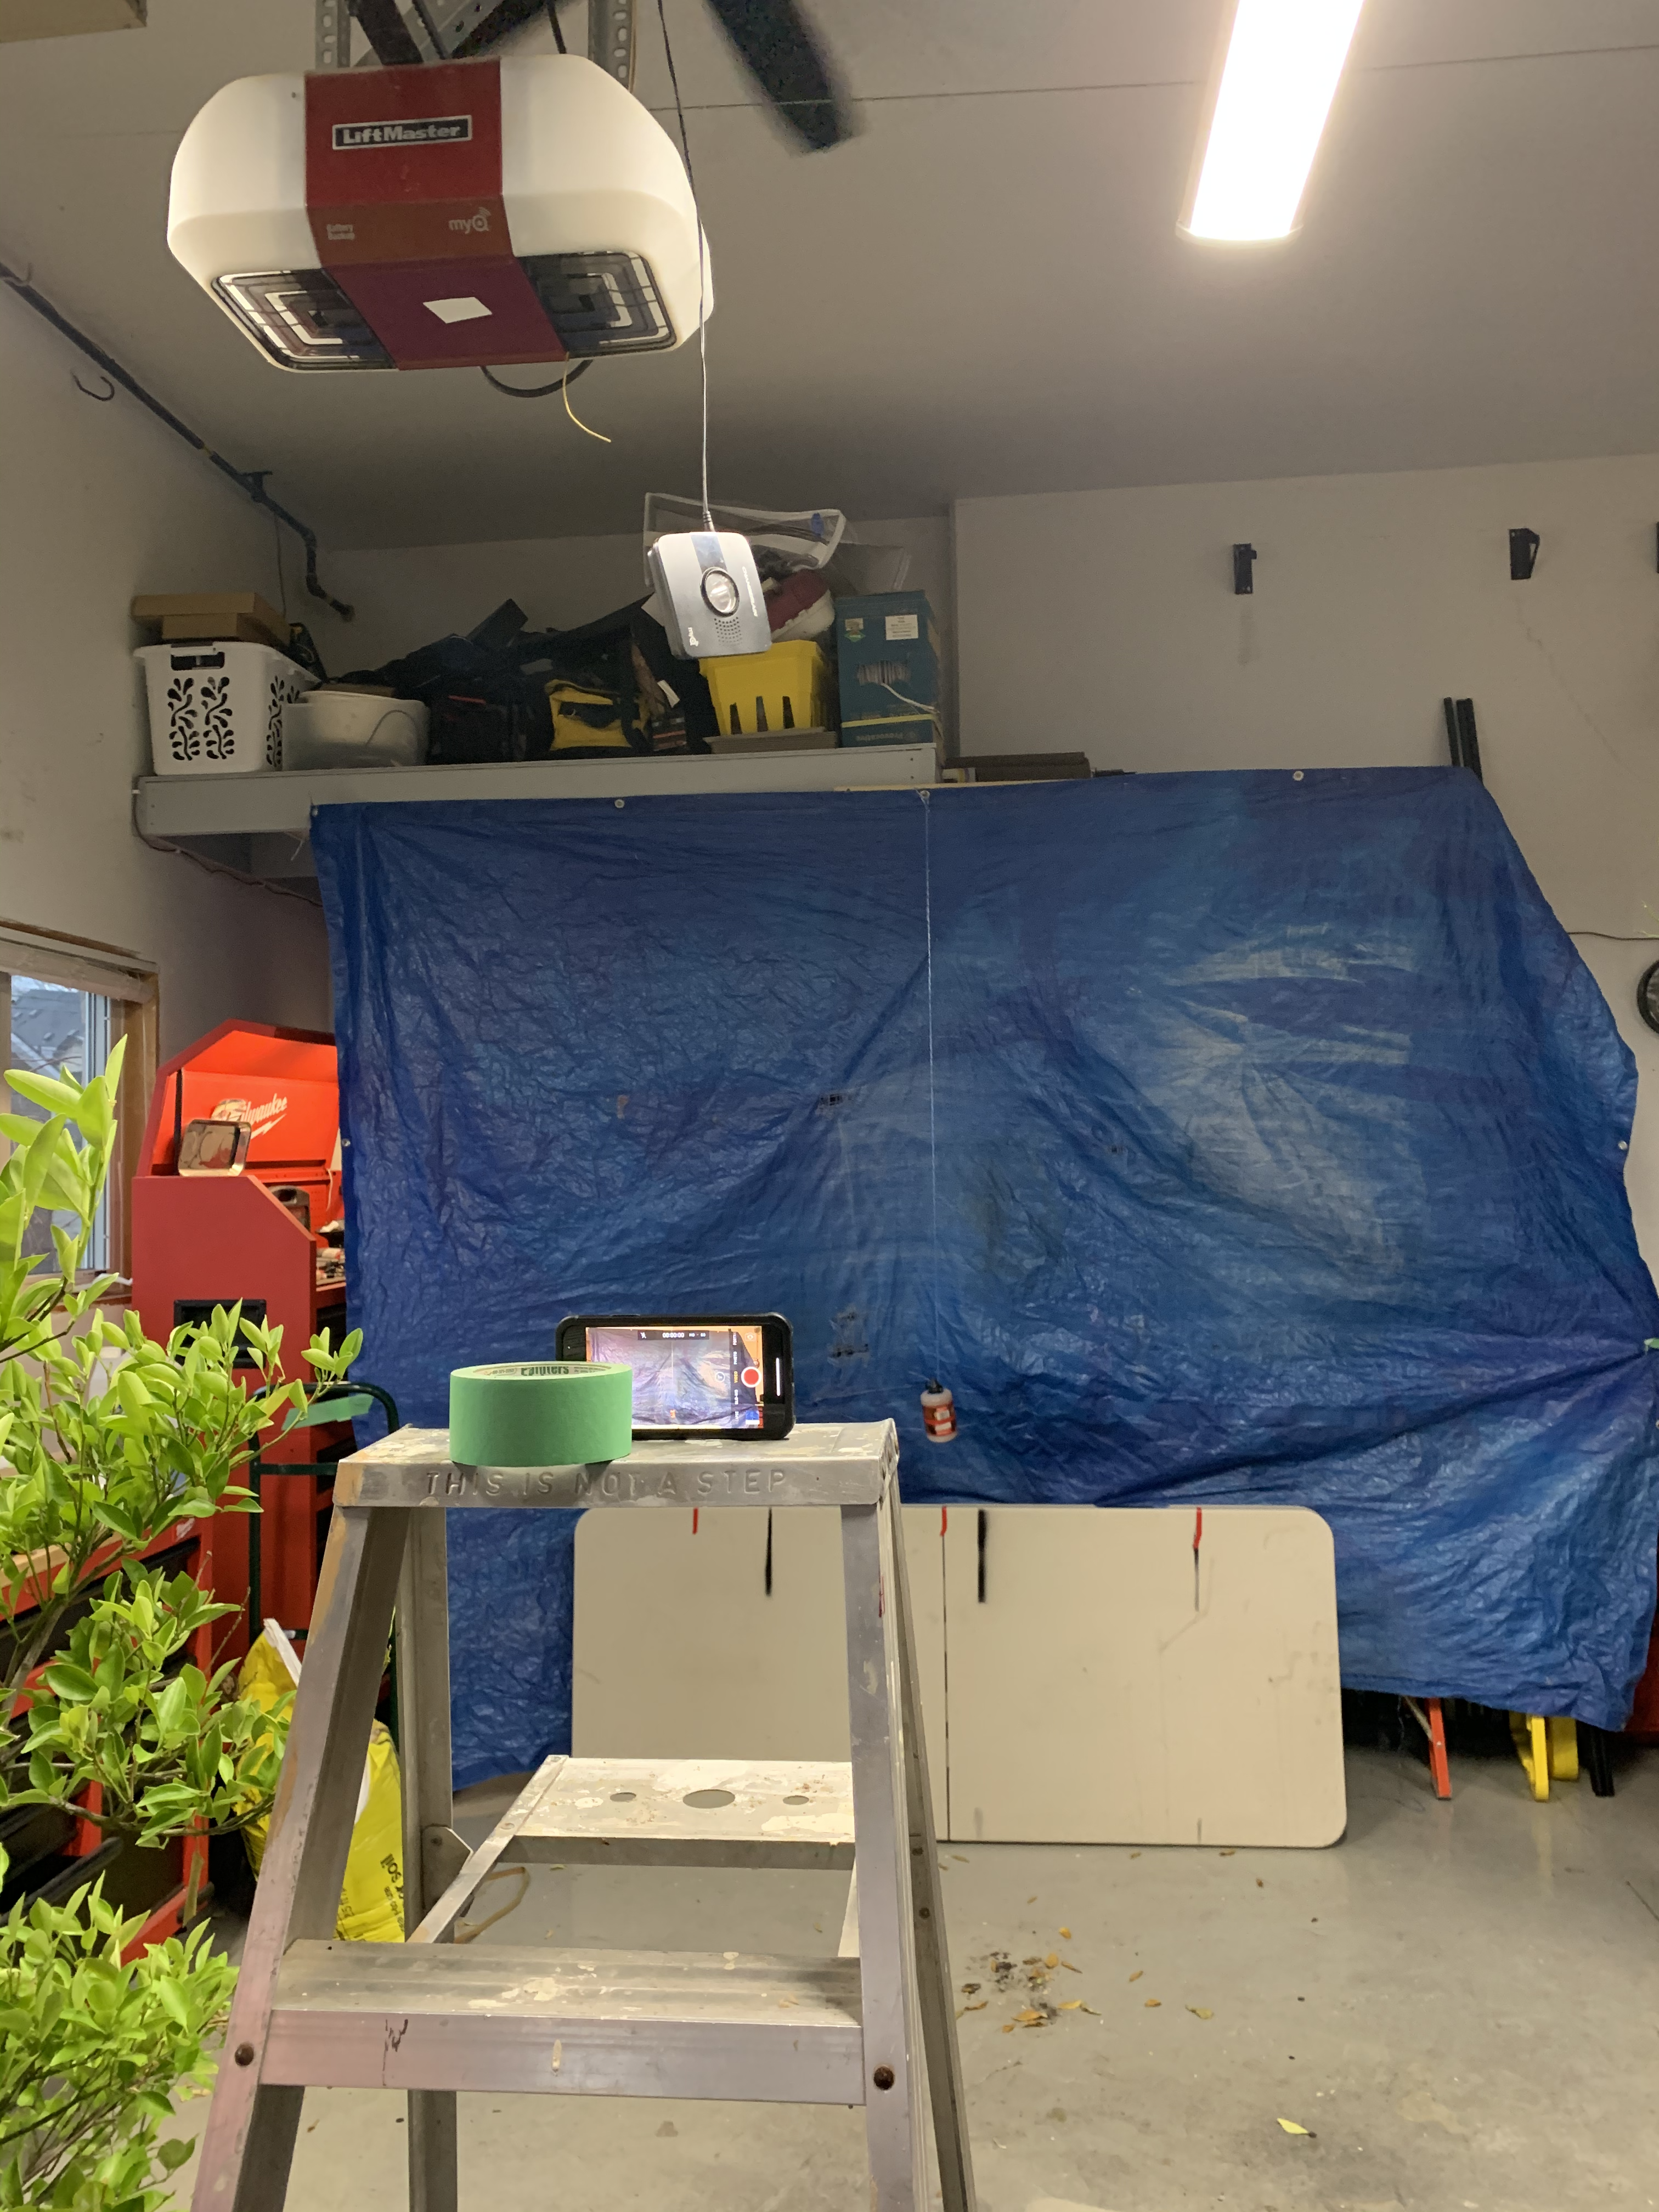
\includegraphics[width=6cm,height=6cm,keepaspectratio]{camerastand.png}
        \caption{View from behind the camera stand, showing the orientation and placement of the entire setup.}
        \label{appendix:camerastand}
    \end{subfigure}
    \newline
    \begin{subfigure}[b]{0.48\textwidth}
        \centering
        \includegraphics[width=6cm,height=6cm,keepaspectratio,angle=270,origin=c]{setup.jpeg}
        \caption{View showing the entire pendulum in equilibrium position. Note that this photo was taken \emph{before} additional length knots were added for Section \ref{section:q4a}.}
        \label{appendix:setup}
    \end{subfigure}
    \hfill
    \begin{subfigure}[b]{0.48\textwidth}
        \centering
        \includegraphics[width=6cm,height=6cm,keepaspectratio]{table.jpeg}
        \caption{View showing the pendulum in equilibrium position above the table marked with tape at 2ft intervals. Note that the equilibrium position lines up with the center of the table.}
        \label{appendix:table}
    \end{subfigure}
    \hfill
    \caption{Photos, group 1.}
\end{figure}
\pagebreak
\begin{figure}[h]
    \centering
    \begin{subfigure}[b]{0.48\textwidth}
        \centering
        \includegraphics[width=6cm,height=6cm,keepaspectratio,angle=270,origin=c]{scale.jpeg}
        \caption{View showing the scale used to mass the bob for Section \ref{section:q4b}.}
        \label{appendix:scale}
    \end{subfigure}
    \hfill
    \begin{subfigure}[b]{0.48\textwidth}
        \centering
        \includegraphics[width=6cm,height=6cm,keepaspectratio]{motionblur.png}
        \caption{View showing the motion blur induced by pendulum velocity at the apex when released from $\theta_0=\pi/2$. Note the length marking.}
        \label{appendix:motionblur}
    \end{subfigure}
    \hfill
    \caption{Photos, group 2.}
\end{figure}

\section{Python Scripts}
\label{appendix:scripts}
\noindent
All scripts have been moved to this project's GitHub repository, at \emph{https://github.com/JLefebvre55/PHY180-Pendulum}. You can find them named appropriately under the "scripts" folder.
\section{Data}
\noindent
On the next page is an example dataset for Section \ref{section:q2} on Q factor. It is abridged and precision-limited for demonstration. Full datasets can be found in the project repository, at \emph{https://github.com/JLefebvre55/PHY180-Pendulum}. You can find them named appropriately under the "data" folder.\medskip\\

    \csvautotabular{abridged.csv}

\bibliographystyle{ieeetr}
\bibliography{references.bib}

\end{document}